\documentclass[twocolumn, 11pt]{article}%
\usepackage{amsmath, amssymb, esint, gensymb, hyperref, mathtools}
\usepackage{graphicx, cuted, geometry, float, scalerel, xcolor, chemfig}

\newcommand\sbullet[1][.5]{\mathbin{\ThisStyle{\vcenter{\hbox{%
  \scalebox{#1}{$\SavedStyle\bullet$}}}}}%
}

\geometry{
    a4paper,
    total={170mm,260mm},
}

\begin{document}

\begin{strip}
  \vspace*{\dimexpr-\stripsep}
  \begin{center}
      \Large\textbf{FISIKA 2}\\
      \large{Pertemuan 2 - Minggu 3 (707101)}\\
      \large{\today}
   \end{center}
\end{strip}

\section{Potensial Listrik}
    \subsection{Energi Potensial Listrik}%
    \subsubsection{Konsep Awal}%
    \begin{itemize}
        \item Medan gaya Coulomb memiliki kemiripan dengan medan gaya Gravitasi, keduanya memiliki bentuk $\displaystyle F \propto\frac12$.
        \item Sebagaimana halnya medan gaya gravitasi, medan gaya Coulomb juga merupakan medan gaya yang bersifat konservatif.
        \item Gerak partikel bermuatan $q$ dalam ruang bermedan listrik dapat dianalogikan dengan gerak partikel bermassa $m$ dalam ruang bermedan gravitasi.
        \item Untuk medan gaya yang bersifat konservatif, dapat didefinisikan suatu besaran skalar yang disebut “potensial”. Terkait medan listrik, fungsi potensial tersebut adalah \textbf{Potensial Listrik} (\textit{electric potential})
    \end{itemize}

    \subsubsection{Energi Potensial Listrik}%
     Untuk memindahkan suatu muatan dari satu tempat ke tempat lainnya dalam pengaruh medan listrik diperlukan sejumlah usaha. Usaha yang dilakukan oleh sebuah gaya adalah:
     \[W_{AB}=\int\limits_A^B \vec F\sbullet[.75]d\vec s=\Delta U\]

    \begin{itemize}
        \item U mengindikasikan fungsi energi potensial bergantung pada posisi.
        \item Gaya Coulomb merupakan gaya konservatif. Untuk medan gaya konservatif, integral lintasannya hanya bergantung pada posisi awal dan akhir.
    \end{itemize}

    Beda energi potensial antara dua buah titik, sama dengan usaha yang diperlukan untuk memindahkan benda melawan medan gaya tersebut.
    \begin{align*}
        U(B)-U(A)&=-W_{AB}\\
        U(B)-U(A)&=-\int\limits_A^B \vec F\sbullet[.75]d\vec s\\
        U(B)-U(A)&=-q\int\limits_A^B \vec E\sbullet[.75]d\vec s\\
        \frac{U(B)}{q}-\frac{U(A)}{q}&=-\int\limits_A^B \vec E\sbullet[.75]d\vec s\\
        V(B)-V(A)&=-q\int\limits_A^B \vec E\sbullet[.75]d\vec s
    \end{align*}

    Ini adalah rumus Energi Potensial Listrik persatuan muatan, atau bisa disebut Potensial Listrik.

    Kenapa negatif? Karena $U(B)$ lebih kecil daripada $U(A)$, maka hasilnya itu negatif. Bayangkan gini, ketika gaya konservatif melakukan sebuah usaha, maka akan terjadi pengurangan energi potensial dan penambahan energi kinetik, namun energi mekaniknya sama (hampir sama dengan potensial gravitasi).
    \begin{center}
        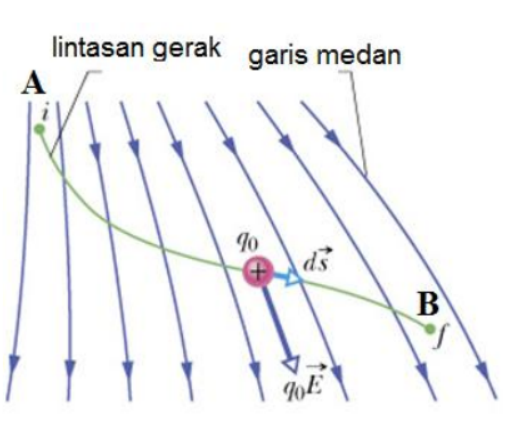
\includegraphics[width=130px]{1.png}
    \end{center}

    Beda potensial listrik antara dua titik bisa didefinisikan dengan usaha yang diperlukan untuk \textbf{melawan} medan gaya Coulomb dalam memindahkan satu satuan muatan dari satu titik ke titik yang lain.

    \subsection{Potensial Listrik}%
    \begin{itemize}
        \item Kita tinjau medan listrik yang ditimbulkan oleh muatan titik
    \end{itemize}

    \begin{align*}
        V(B)-V(A)&=-q\int\limits_A^B \vec E\sbullet[.75]d\vec s\\
        &=-kQ \int\limits_{r_A}^{r_B}\frac1{r^2}\hat r \sbullet[.75]dr\ \hat r\\
        &=k\frac{Q}r \bigg|_{r_A}^{r_B}\\
        &=kQ\left(\frac1{r_B} - \frac1{r_A}\right)
     \end{align*}

     \begin{itemize}
         \item Jika diambil acuan di suatu titik tertentu (misal $\infty$) dengan potensial tertentu (misal 0), maka..
     \end{itemize}

     \begin{align*}
         0-V(A)&=k\frac{Q}{r} \bigg|_{r_A}^{\infty}\\
               &= kQ\left( \frac1{\infty}-\frac1{r_A} \right)\\
         V(A) &= k\frac{Q}{r_A}
     \end{align*}

     Itu adalah Potensial listrik pada jarak $r_A$ dari suatu muatan $Q$.
     \begin{center}
         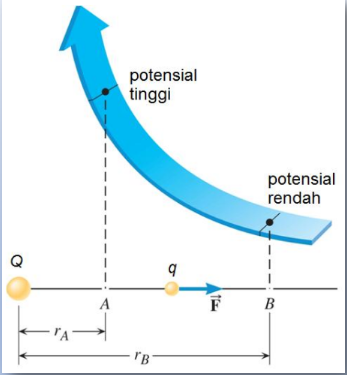
\includegraphics[width=100px]{2.png}
         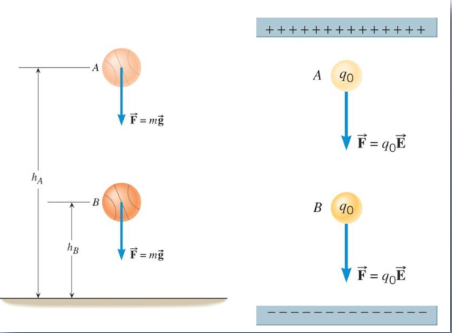
\includegraphics[width=140px]{3.png}
     \end{center}

     Gambar 2 ini merupakan gambaran analogi antara potensial listrik dengan potensial gravitasi.

     \subsubsection{Definisi}%
     \begin{itemize}
         \item Besaran potensial listrik di suatu tempat hanya mempunyai makna jika dibandingkan dengan potensial di tempat lain.
         \item Jadi yang mempunyai makna fisis adalah \textbf{beda potensial} (ada tempat yang digunakan sebagai acuan)
         \item Beda potensial listrik antara dua buah titik merupakan usaha persatuan muatan yang diperlukan untuk memindahkan benda dari satu titik ke titik lainnya melawan medan gaya Coulomb.
         \item Potensial listrik di suatu titik sama dengan usaha persatuan muatan yang diperlukan untuk memindahkan muatan dari titik acuan (biasanya diambil pada $\infty$) ke titik yang dimaksud.
     \end{itemize}

     \subsubsection{Potensial Listrik Oleh Muatan Titik}%
     \begin{itemize}
         \item Jika terdapat beberapa muatan titik, maka potensial listrik total di suatu tempat dapat diperoleh menggunakan prinsip superposisi (penjumlahan) potensial listrik yang disebabkan oleh masing-masing muatan titik.
         \item Potensial listrik adalah besaran \textbf{skalar}.
         \item Satu volt sama dengan Joule per Coulomb. $\displaystyle V=\frac{J}{C}$
     \end{itemize}

     \begin{center}
         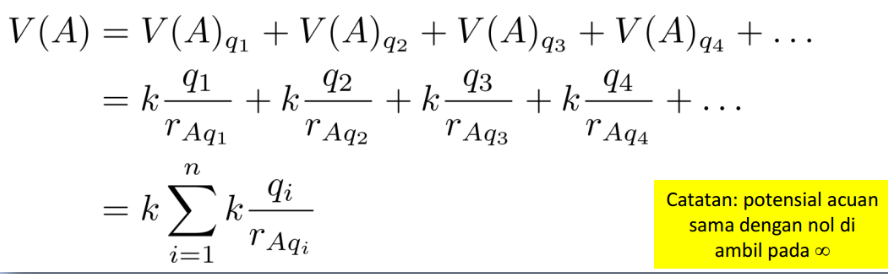
\includegraphics[width=220px]{4.png}
     \end{center}

     $V(A)$ menotasikan potensial listrik di titik $A$, sedangkan $r_{Aqi}$ ialah jarak dari muatan $q_1$ ke titik $A$ tersebut.\\

     \textbf{Contoh:}

     \begin{enumerate}
         \item Tentukanlah potensial listrik di titik A dan B akibat kedua muatan
         \begin{center}
            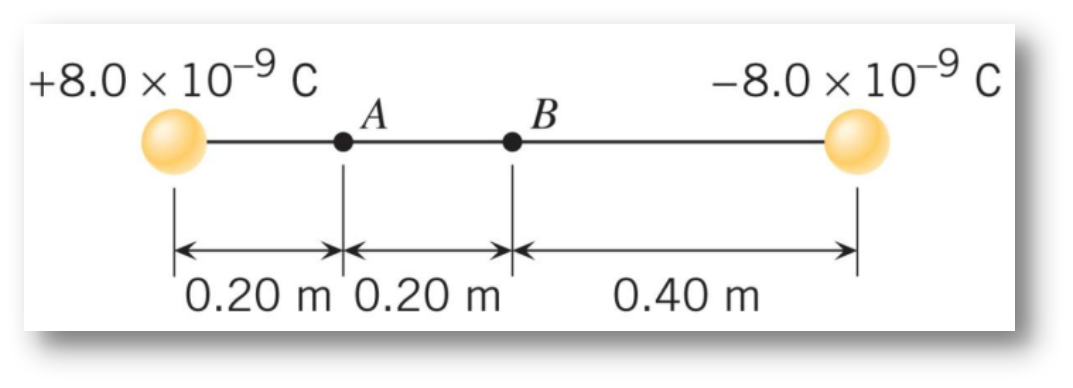
\includegraphics[width=200px]{5.png}
         \end{center}

         \item Tentukanlah energi potensial sistem tiga muatan berikut, jika $q_1=+q$ , $q_2=-4q$ dan $q_3=+2q$ dengan $d=12 cm$ dan $q=150 nC$
             \begin{center}
                    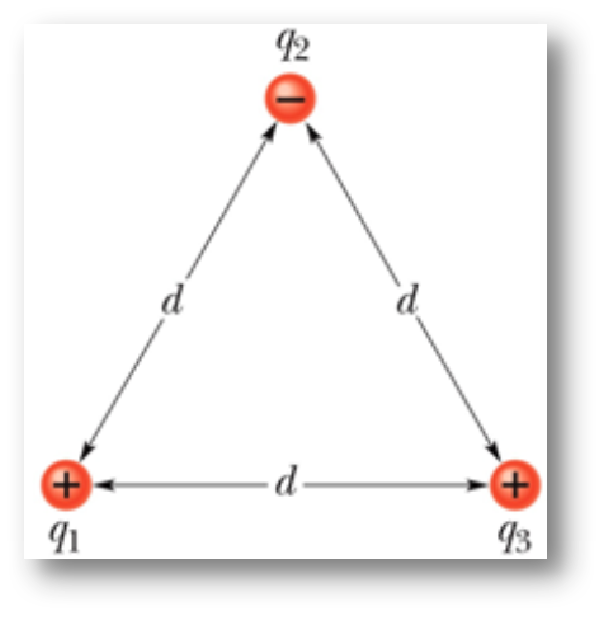
\includegraphics[width=110px]{6.png}
             \end{center}
     \end{enumerate}

     \textbf{Jawaban:} 
     \begin{enumerate}
         \item 
             \begin{itemize}
                 \item Potensial di Titik A
                     \begin{align*}
                         V_A&=k\frac{Q_1}{r_{A1}}+k\frac{Q_2}{r_{A2}}\\
                            &=k\left(\frac{8\times10^{-9}}{0.2} +\frac{-8\times10^{-9}}{0.6}\right)\\
                            &\approx 240
                     \end{align*}
             \end{itemize}
             \begin{itemize}
                 \item Potensial di Titik B
                     \begin{align*}
                         V_A&=k\frac{Q_1}{r_{B1}}+k\frac{Q_2}{r_{B2}}\\
                            &=k\left(\frac{8\times10^{-9}}{0.4} +\frac{-8\times10^{-9}}{0.4}\right)\\
                            &= 0
                     \end{align*}
             \end{itemize}
        \item 
            Energi potensial sistem sama dengan usaha yang diperlukan untuk menyusun muatan-muatan tersebut
            \begin{align*}
                U&=U_{12}+U_{13}+U_{23}\\
                 &=q_2V_{q_1 q_2}+q_3V_{q_1 q_3}+q_2V_{q_2 q_3}\\
                 &=k\left(\frac{q_1q_2}{r_{12}}+\frac{q_1q_3}{r_{13}}+\frac{q_2q_3}{r_{23}}\right)\\
                 &=k\left(\frac{-4q^2}d + \frac{2q^2}d + \frac{-8q^2}d \right)\\
                 &= -10k\frac{q^2}d
            \end{align*}
     \end{enumerate}

     \subsubsection{Permukaan Ekuipotensial}%
     \begin{itemize}
         \item Posisi dalam ruang yang mempunyai nilai potensial sama membentuk suatu \textbf{permukaan ekuipotensial} (kasus 3D) atau \textbf{garis ekuipotensial} (kasus 2D).
         \item Untuk muatan titik dalam ruang (3D), permukaan ekuipotensial nya berbentuk permukaan bola.
         \item Untuk muatan titik dalam bidang (2D), garis ekuipotensial nya berupa lingkaran.
     \end{itemize}

     \begin{center}
         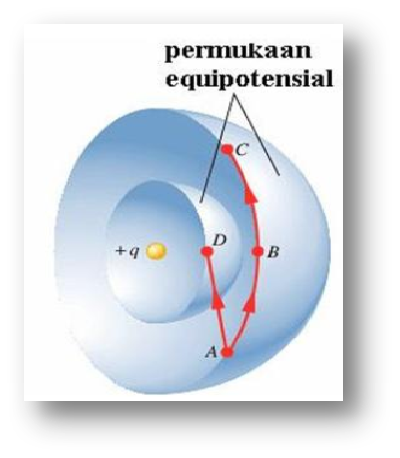
\includegraphics[width=100px]{7.png}
         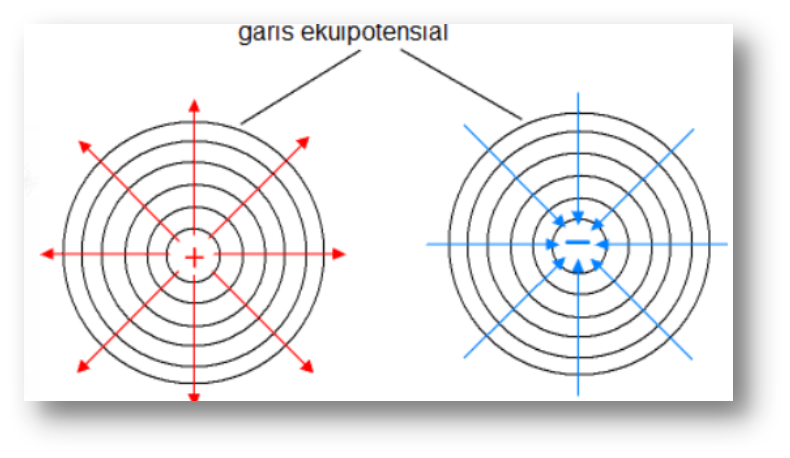
\includegraphics[width=130px]{8.png}
         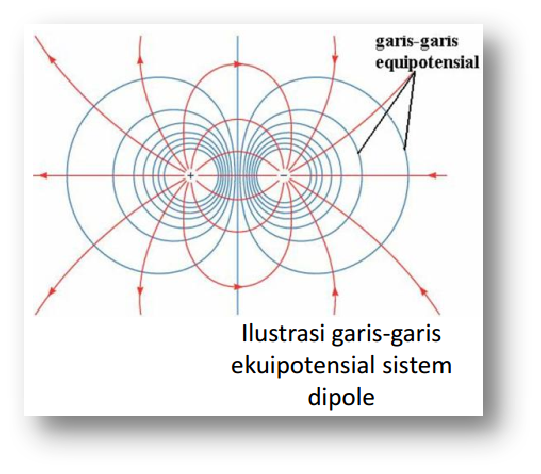
\includegraphics[width=130px]{9.png}
     \end{center}

     \subsubsection{Hubungan Antara Potensial Listrik dan Medan Listrik}%
     \begin{itemize}
         \item Jika diketahui medan listrik $\vec E$, maka potensial listrik dapat diperoleh dengan mengingat pengertian (energi) potensial listrik sebagai berikut:
             \[ \Delta V=V(B)-V(A)=-\int\limits_A^B \vec E\sbullet[.75] d\vec s\]
         \item Untuk medan listrik yang konstan dan searah maka akan diperoleh:
             \begin{align*}
                 \Delta V&=V(B)-V(A)\\
                         &=-\int\limits_A^B \vec E\sbullet[.75] d\vec s\\
                         &=-E(\Delta s_{AB})\\
                 E&=-\frac{\Delta V}{\Delta s}
             \end{align*}
         \item Untuk medan listrik konstan dan arah perpindahan muatan yang tegak lurus, telah diperoleh:
             \[ E= \frac{\Delta V}{\Delta s} \]
         \item Komponen vektor medan listrik $\vec E$, pada suatu arah tertentu sama dengan \textbf{negatif laju perubahan} (gradien) potensial listrik terhadap jarak pada arah tersebut
             \[E=\frac{\partial V}{\partial s} \]
        \item Atau kalau dalam koordinat kartesian adalah
            \[\vec E=-\frac{\partial V}{\partial x}\hat i - \frac{\partial V}{\partial y}\hat j - \frac{\partial V}{\partial z}\hat k = \vec\nabla V \]
            \[ E_x=\frac{\partial V}{\partial x}\ ;\ E_y=\frac{\partial V}{\partial y}\ ;\ E_z=\frac{\partial V}{\partial z} \]
     \end{itemize}

     \subsubsection{Potensial Listrik Akibat Dipole Listrik}%
     Dipole adalah dua muatan titik dengan besar yang sama tapi dengan jenis yang berbeda
     \[V_p=k\left(\frac{+q}{r_+} + \frac{-q}{r_-}\right) = kq\left(\frac{r_- - r_+}{r_+ r_-}\right) \]
    
     Untuk kasus titik P yang jauh dari dipole tersebut $(r >> d)$ dapat digunakan pendekatan
     \[ r_- \approx r_+ \approx r\text{ dan } r_--r_+ \approx d\cos\theta\]
     Sehingga
     \[ V_P\approx kq\left(\frac{d\cos\theta}{r^2}\right) \]
    
     Apabila $p=qd$, maka
     \[ V_P \approx k\left(\frac{p\cos\theta}{r^2}\right) \]

     \textbf{$p$ menotasikan momen dipole} 

     \begin{center}
         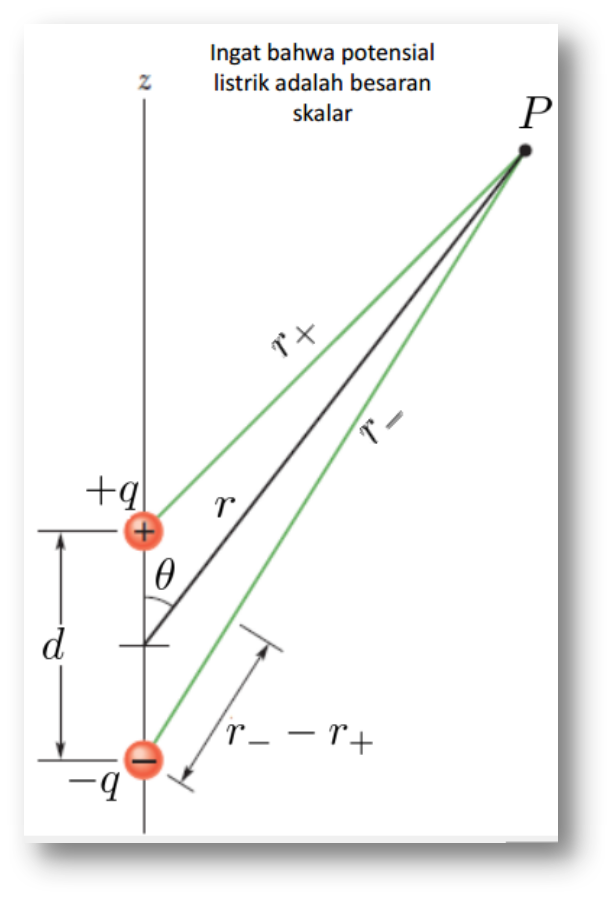
\includegraphics[width=100px]{10.png}
     \end{center}

     \textbf{Contoh:} 
     \begin{itemize}
         \item Potensial listrik dalam ruang yang ditimbulkan oleh muatan titik $q$ di $(x_0,y_0,z_0)$ dinyatakan dengan
             \begin{align*}
             V(x,y,z)=\frac{kq}{\sqrt{(x-x_0)^2+(y-y_0)^2+(z-z_0)^2}}
             \end{align*}
             Tentukanlah bentuk vektor medan listrik $\vec E(x,y,z)$ dalam ruang yang ditimbulkan oleh muatan titik tersebut.
     \end{itemize}

     \textbf{Jawaban:} 
     \begin{center}
         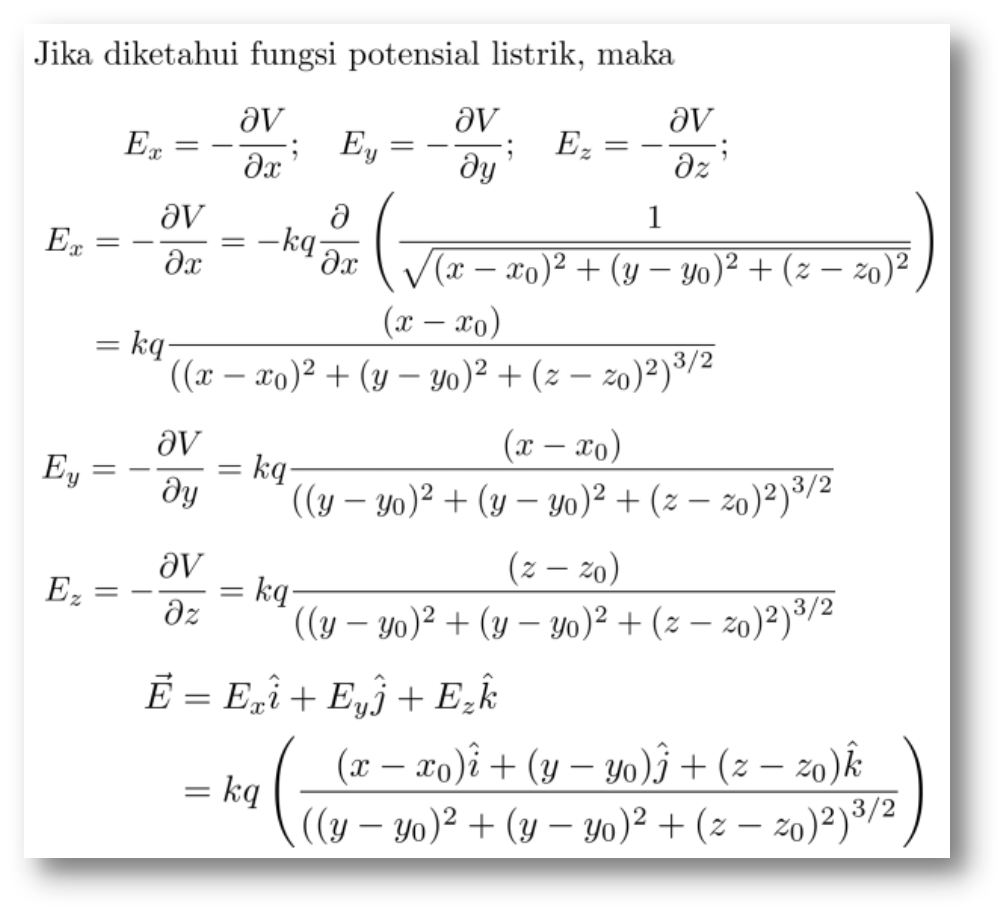
\includegraphics[width=230px]{11.png}
     \end{center}

     \subsection{Potensial Listrik Akibat Muatan Terdistribusi Kontinu}%
     \begin{itemize}
         \item Muatan terdistribusi dalam satu dimensi (1D); rapat muatan persatuan panjang ($\lambda$), $\Rightarrow$ batang bermuatan, cincin.
         \item Muatan terdisribusi dalam dua dimensi (2D); rapat muatan persatuan luas ($\sigma$) $\Rightarrow$ permukaan/ lempengan bermuatan.
         \item Muatan terdistribusi dalam tiga dimensi (3D); rapat muatan persatuan volume ($\rho$) $\Rightarrow$ bola/ silinder/ kubus bermuatan.
     \end{itemize}

     \subsubsection{Batang Lurus}%
     \begin{center}
         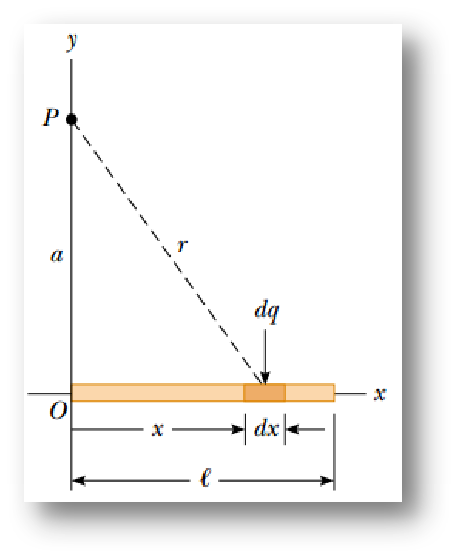
\includegraphics[width=170px]{12.png}
     \end{center}
     \begin{itemize}
         \item Potensial listrik pada titik $P$ yang disebabkan oleh muatan serba sama pada batang dari $0$ sampai $l$, dapat dituliskan sebagai:
             \[dC=k\frac{dq}r=k\frac{\lambda\ dx}{\sqrt{x^2+a^2}} \]
        \item Dengan melakukan integrasi dan mengaplikasikan syarat batasnya, dapat diperoleh:
            \begin{align*}
                V&=k\int\limits_0^l \frac{\lambda\ dx}{\sqrt{x^2+a^2}}\\
                 &=k\lambda\ln\left(x+\sqrt{x^2+a^2}\right)\bigg|_0^l\\
                 &=k\lambda\ln\left(\frac{l+\sqrt{l^2+a^2}}a\right)\\
                V&=k\lambda\ln\left(\frac{l+\sqrt{l^2+a^2}}a\right)
            \end{align*}
     \end{itemize}

     \subsubsection{Cincin}%
     \begin{center}
         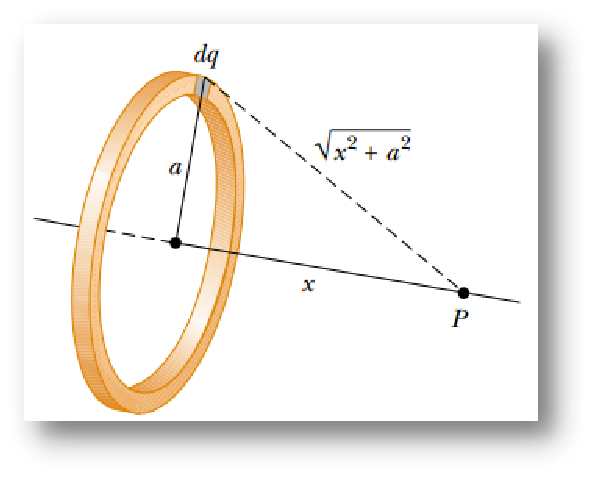
\includegraphics[width=170px]{15.png}
     \end{center}
     \begin{itemize}
         \item Potensial listrik di titik $P$ yang disebabkan oleh muatan $q$ pada cincin dideskripsikan oleh:
             \[V=k\int\frac{dq}r=k\int\frac{dq}{\sqrt{x^2+a^2}} \]
        \item Karena setiap elemen $dq$ memiliki jarak yang sama dengan $P$, maka potensial listrik di $P$ dapat ditulis:   
            \[V=\frac{k}{\sqrt{x^2+a^2}}\int dq=\frac{kQ}{\sqrt{x^2+a^2}}\]
        \item Apabila dijadikan medan listrik, maka
            \begin{center}
                
\includegraphics[width=140px]{16.png}
            \end{center}
     \end{itemize}

     \subsubsection{Piringan}%
     \begin{center}
         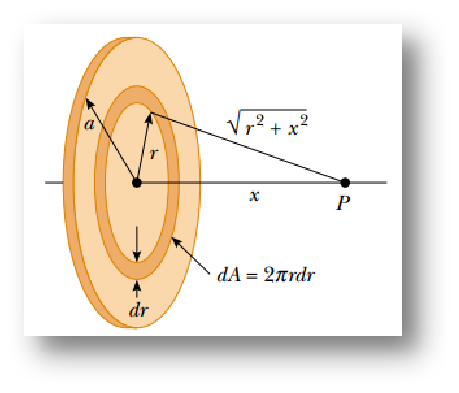
\includegraphics[width=170px]{13.png}
     \end{center}
     Potensial listrik pada piringan yang memiliki muatan yang seragam

     \begin{align*}
         V&=k\int\frac{dq}r\\
          &=k\int\frac{\sigma2\pi r\ dr}{\sqrt{x^2+r^2}}\\
          &= \pi\sigma k\int\limits_0^a \frac{2r\ dr}{\sqrt{x^2+r^2}}
     \end{align*}
     
     misalkan $\displaystyle u=(x^2+r^2)$, maka $du=r\ dr$

     Sehingga
     \[ \int(x^2+r^2)^{-1/2} 2r\ dr = \int u^{-1/2}du=2u^{-1/2}\]

     Jadi
     \[V=2\pi\sigma k(x^2+r^2)^{1/2}\bigg|_0^a \]

     Dengan demikian potensial listrik di titik P adalah
     \[ V=2\pi\sigma k \left[(x^2+a^2)^{1/2}-x \right] \]

     Medan listrik di titik P bisa dihitung dengan
     \[E_x=-\frac{dV}{dx}=2\pi\sigma k\left[1-\frac{x}{(x^2+a^2)^{1/2}}\right] \]

     \subsubsection{Bola Isolator}%
     Bola pejal dengan rapat muatan yang merata, pada permukaan bola tersebut memiliki muatan $Q$.
     \begin{center}
         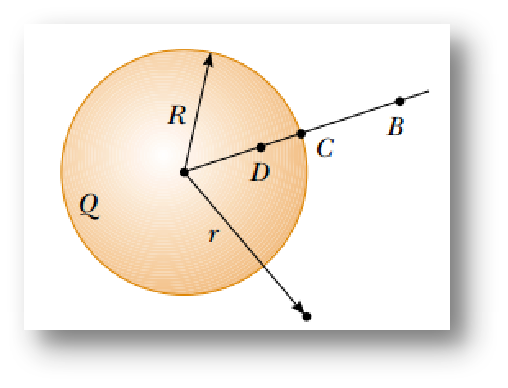
\includegraphics[width=150px]{14.png}
     \end{center}
 \[V(B)=\frac{kQ}{r_B}\ \text{ (untuk }r>R) \]
 \[V(C)=\frac{kQ}{r_C}\ \text{ (untuk }r=R) \]
 \[V(D)=\frac{kQ}{2R} \left(3-\frac{r_D}{R^2}\right)\ \text{ (untuk }r<R) \]
     
    \subsubsection{Bola Konduktor}%
     \begin{center}
         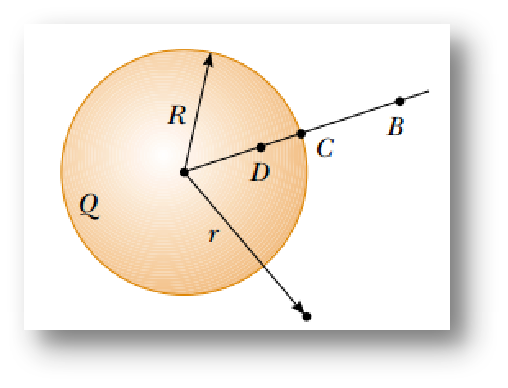
\includegraphics[width=150px]{14.png}
     \end{center}
    Karena medan listrik pada dalam konduktor adalah nol, maka potensial listriknya sama dengan di permukaannya
 \[V(C)=\frac{kQ}{r_C}\ \text{ (untuk }r=R) \]
    
    \subsubsection{Silinder}%
    \begin{itemize}
        \item Silinder konsentris dengan jari-jari $a_1$ dan $a_2$ yang memiliki muatan masing-masing $+Q$ dan $–Q$, sebagaimana gambar berikut ini
            \begin{center}
                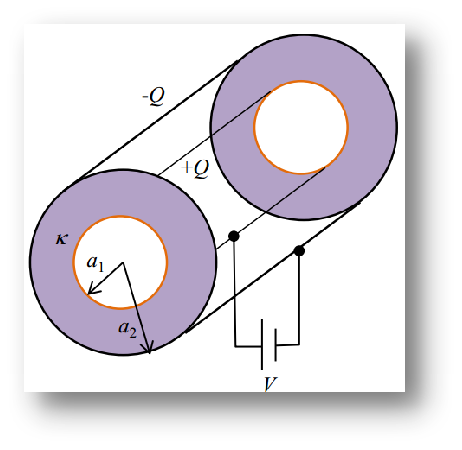
\includegraphics[width=150px]{17.png}
            \end{center}
        Maka beda potensial antara keduanya ialah
        \begin{align*}
            V(a_1)-V(a_2) &= \frac{\lambda}{2\pi\epsilon_0}\ln\left(\frac{a_2}{a_1}\right)\\
            V(a_1)&=V(a_2)+\frac{\lambda}{2\pi\epsilon_0}\ln\left(\frac{a_2}{a_1}\right)
        \end{align*}
    \end{itemize}
\end{document}
